% \begin{abstract}

The validation of ground motion synthetics has received increased attention over the last few years due to advances in physics-based deterministic and hybrid simulation methods. Validation of synthetics is necessary in order to determine whether the available simulation methods are capable of faithfully reproducing the characteristics of ground motions from past earthquakes. Some validation methods use filters to evaluate the quality of the fit between synthetics and data within different frequency bands. This is done, primarily, to weight the contribution of different wavelengths so that low frequencies are given more weight than high frequencies. One particular method of interest is the goodness-of-fit (GOF) criterion introduced by Anderson (2004). In this method, the degree of similarity between two signals is quantified by means of a set of ten (error) metrics which are projected on a 0?10 scoring scale. These metrics are based on ground motion characteristics commonly used in seismology and earthquake engineering. The scores are used to evaluate each given pair of signals in the three components of motion and within different frequency ranges. The scores of each frequency band, component, and metric are then combined to obtain a final GOF score. In this paper we study the sensitivity of the GOF scores, and thus the sensitivity of the validation itself, to the filtering process when different filter parameters are considered. Our initial analysis of results shows that GOF methods are susceptible to the design of filters. The filter?s order, for instance, seems to significantly affect the interpretation of the validation especially for metrics that are time-dependent (e.g., peak ground response). We evaluate the implications of the variability in GOF scores on the 60 randomly generated (white noise) waves. We calculated the best parameters to each filter through Genetic Algorithm. We test best sets of parameters on two case studies of the 2008 Mw 5.4 Chino Hills earthquake, and Broadband Platform, investigate the sensitivity of GOF criteria to the type of filters used to decompose the signals. We analyze the consistency and correlation of the results obtained using various metrics by means of a filtering fitting function. Our work indicates that elliptic infinite impulse response filters lead to more reliable results, over other more commonly used filters; and the filtering parameters are mainly dependent on filtering bandwidth. We provide relationships to select the most accurate parameters of elliptic filter.

% \end{abstract}

\section{Introduction}

With recent advances in earthquake ground motion simulation using physics-based methods and hybrid approaches \citep[e.g.,][]{Bielak_2010_GJI,Graves_2010}, verification and validation (V\&V) of synthetics have become increasingly relevant. V\&V imply processing signals in preparation to perform qualitative and quantitative comparisons. We are particularly interested in investigating the effect that different filtering procedures and parameters can have on quantitative validations done using the goodness-of-fit (GOF) method introduced by Anderson (2004). In this method, the degree of similarity between two signals is quantified by means of a set of ten (error) metrics, labeled C1 through C10. These metrics include ground motion characterization parameters commonly used in seismology and earthquake engineering. The quantitative comparisons are projected on a 0?10 scoring scale, where a score of 10 corresponds to a perfect match. When using Anderson?s method, signal pairs are compared by component of motion and at different frequency ranges to weight the contribution of different wavelengths so that low frequencies are given more weight than high frequencies.
The scores of each frequency band, component, and metric are then combined to obtain a final GOF value. \citet{Khoshnevis_2015} found that filtering, in particular, can play a significant role in the output of the GOF scores. Also they showed that the variation of the order of a finite impulse response (FIR) filter has a substantial influence on the GOF scores, especially on those metrics that are strongly time dependent. Therefore, among the metrics considered in the GOF method, the Arias intensity score, and the peak acceleration, velocity and displacement scores are most sensitive; followed by the scores derived from the energy integral, energy duration, Arias duration, cross correlation, response spectra and Fourier spectra; with the latter being the least sensitive of all.



% \begin{figure} [H]
% \begin{center}  
% 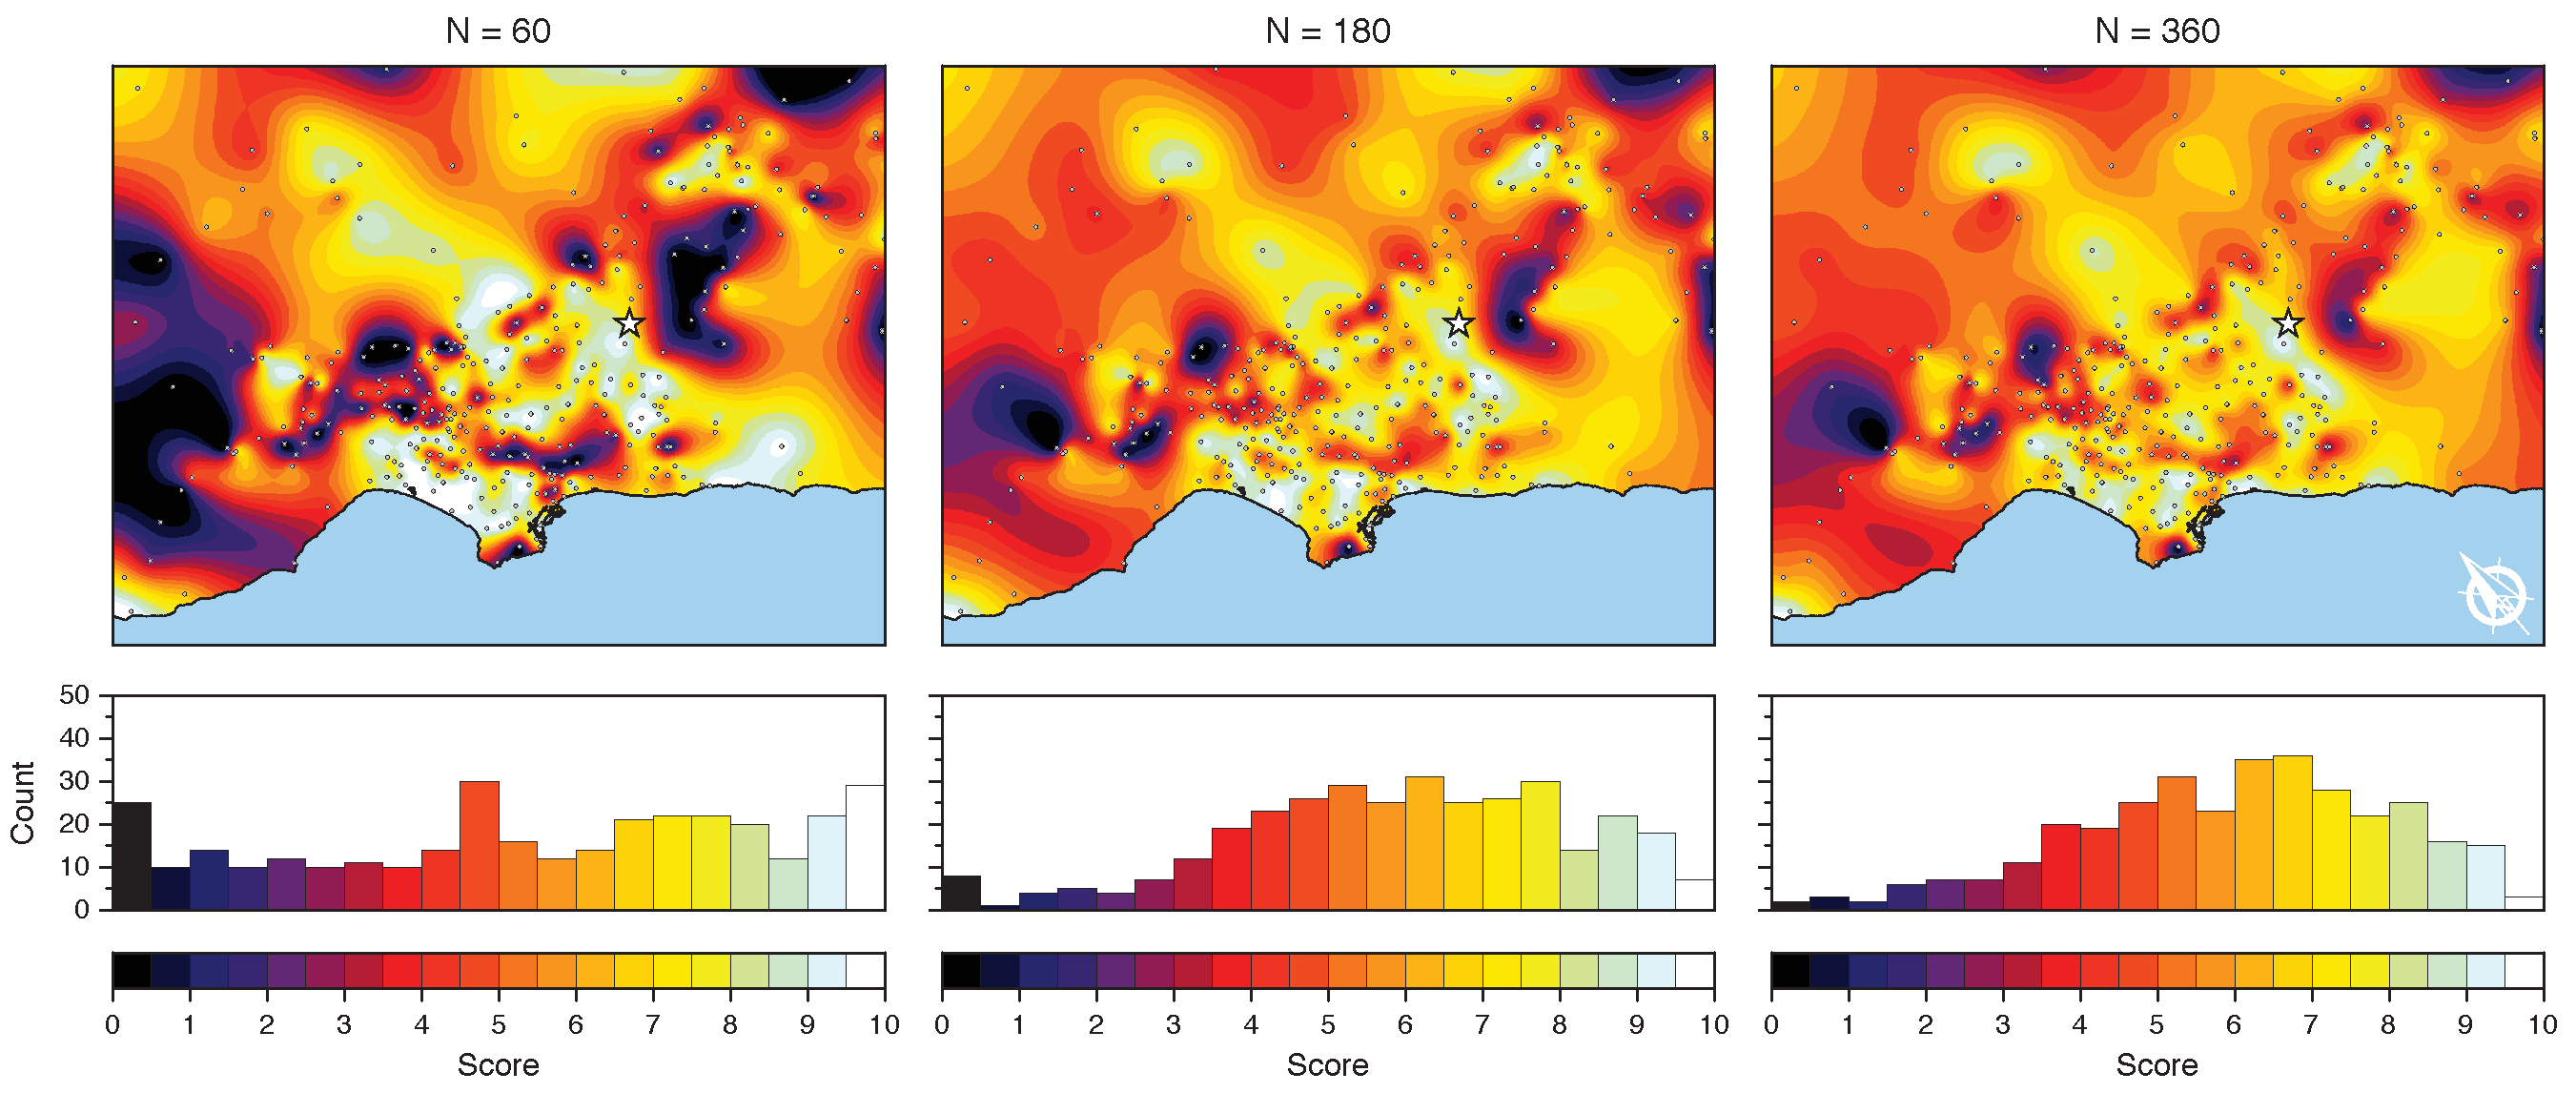
\includegraphics[scale=0.36]{figures/pdf/figure1.pdf} 
% \caption{Variation of PGA GOF scores for the case study of the 2008 Mw 5.4 Chino Hills, California, earthquake using FIR Chebyshev filters with order N = 60 (left), 180 (center) and 360 (right). Top frames show contours drawn based on GOF values derived from 336 stations with records used for the comparisons against synthetics from \citet{Taborda_2013_BSSA}. Bottom frames show histogram distributions in the GOF scale introduced by \citet{Anderson_2004}.}
% \end{center}   
% \end{figure}



% \begin{figure} [H]
% \begin{center}  
% 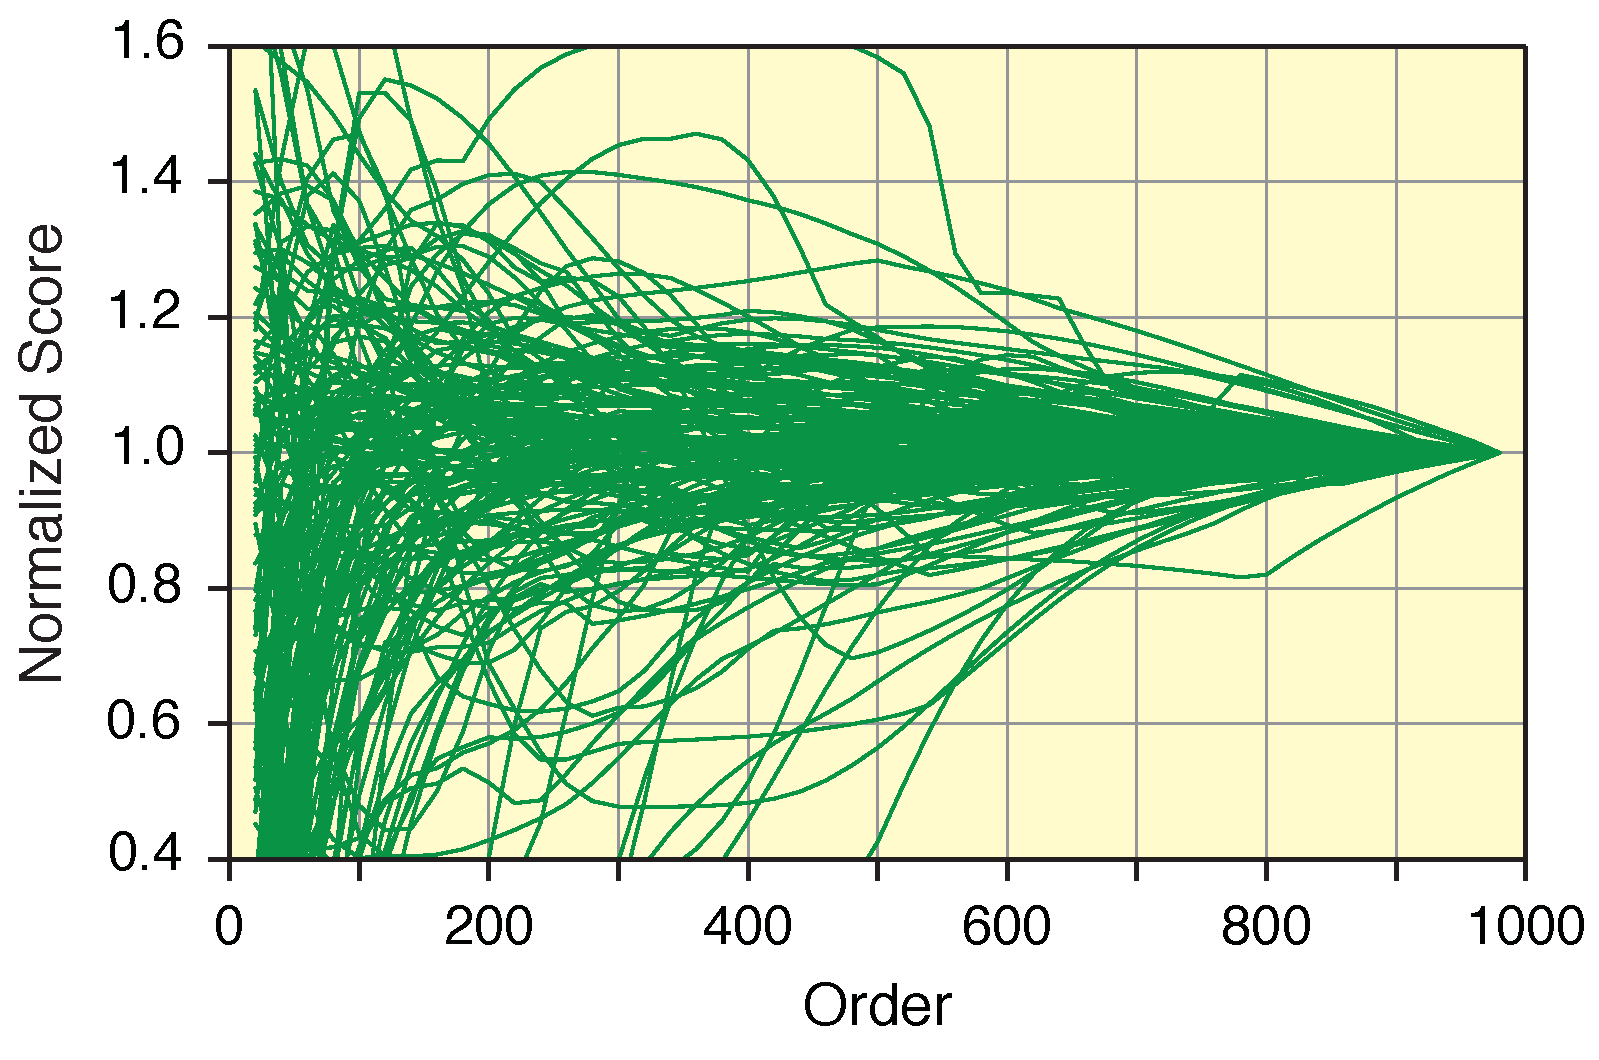
\includegraphics[scale=0.4]{figures/pdf/figure2.pdf} 
% \caption{Variation of PGA GOF scores with increasing order of FIR Chebyshev  filter for the same 336 stations used for the  validation of the Chino Hills earthquake simulation.}
% \end{center}   
% \end{figure}


% Figure 2 shows the variation of PGA GOF scores with filter order for the same 336 signal pairs from the Chino Hills simulation. Each score trend is normalized with respect to the value obtained with the highest order. Despite the chosen normalization, the substantial variability over the range of order values suggests that, even for higher order filters, there is not one stable score. Using different types of filters can also be influential on the results. \citet{Khoshnevis2015} implemented a Chebyhsev I infinite impulse response (IIR) filter, instead. As we will explain in greater detail below, IIR filters have sharper cutoffs at the corner frequencies, yet they present ripples in the passband. Figure 3 shows the frequency response of a FIR and an IIR bandpass filter and a comparison of a portion of the Fourier amplitude spectra around the cutoff frequency of a signal filtered using these two type of filters, along with the unfiltered signal. As it can be seen in this figure, the amplitudes of the FIR filtered signal and the original signal are nearly identical within a portion of the passband, but they differ from each other over a wider transition zone than that of the IIR filter.
% In turn, the IIR filter does not have a perfect match within the passband, but it exhibits a sharper decay past the cutoff frequency. Arguably, for most applications, these differences are minor and inconsequential. Their effect on GOF scores used for validation may, however, become relevant, especially in the absence of a well-accepted standard. 

% \begin{figure} [H]
% \begin{center}  
% 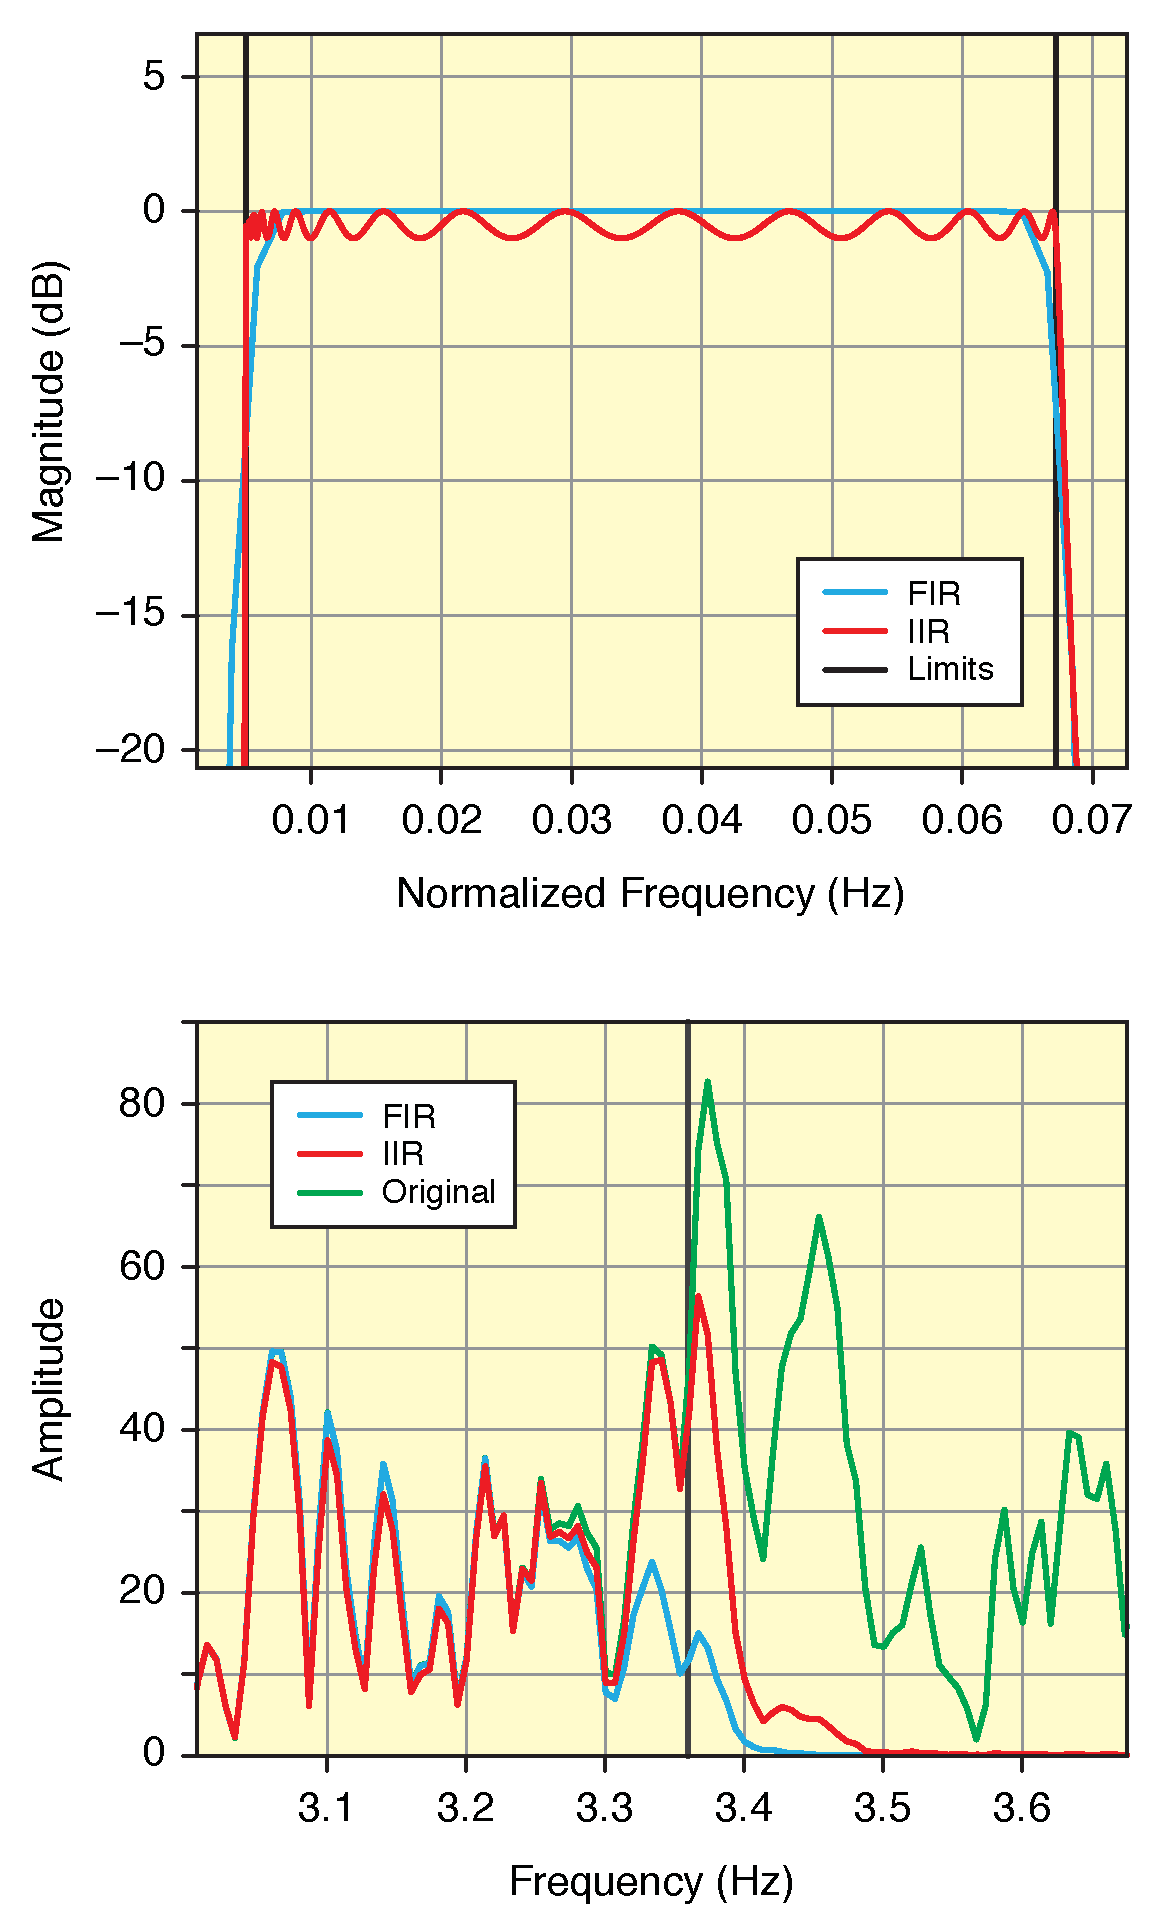
\includegraphics[scale=0.4]{figures/pdf/figure3.pdf} 
% \caption{Comparison between FIR and IIR filters. Top: amplitude response (dB) of the bandpass filters' design in normalized frequency for corner frequencies equal to 0.1 and 0.3 of the maximum frequency. Bottom:
% detail of a Fourier amplitude spectra around the upper cutoff frequency of a signal filtered with both IIR and FIR filters (the original signal is also included).
% }
% \end{center}   
% \end{figure}

% Moreover, since simulations involve numerous unknowns and assumptions, it is imperative to minimize the additional uncertainties that post-processing of the data may have on the analysis of results. In this paper we seek to contribute to reducing such additional uncertainties by investigating the characteristics of filters used in ground motion signal processing for validation purposes. While it would be difficult to decide on a final ideal filter, it is desirable to define a filter that can be used consistently in validation studies with minor effects on the analysis. Here, we contribute to such an objective. We review the characteristics of the most commonly used FIR and IIR filters, and make initial recommendations on the selection of suitable filter for ground motion simulation validation. Among IIR filters Butterworth filter is more common to use in seismological studies \citep{Ma_2008,Lee_2014,Olsen_2003}. For many of application the filter presents good results. The Butterworth filter is defined based on having uniform sensitivity for wanted frequencies and completely reject unwanted frequencies. Designing filter is trade of between parameters of passband, transition zone, and stopband(i.e. filter order, allowable ripple, min stop band attenuation). Butterworth filter even though completely preserve the passband magnitude and almost completely reject the stop band however it is not successful in transition zone. Even though Butterworth filter designed to have uniform sensitivity of wanted frequency, we can decrease the allowable ripple in elliptic filter to have almost uniform results. However we may not able to decrease the transition zones width in Butterworth filter through commonly used signal processing packages. These transition zones are very important when we are studying very narrow bands. \citet{Oppenheim_1989} suggests using elliptic filter in order to have accurate results in both inside and outside of the band. \citet{Khoshnevis_2015} in a preliminary study shows that elliptic filter gives good results. Elliptic filter can take more input parameter as factors for controlling the filter behavior.   In this paper we are presenting best parameters based on bandwidth to use in filtering process of validation studies. 

% \section{Finite and Infinite Impulse Response filters}

% Filters are a particularly important class of linear time-invariant systems. Strictly speaking, the term frequency-selective filter suggests the existence of a system that passes certain frequency components and rejects all others. In practice, however, filters are far from ideal, and there are different kinds of filters, each of them with advantages and disadvantages. To aid the discussion, in Figure 4, we show the main characteristics of a low-pass filter in the frequency domain. Here, d1 is the maximum ripple?s amplitude in the passband, d2 is maximum ripple?s amplitude in the stopband, wp is the normalized cut-off frequency in the passband, and ws is the normalized cut-off frequency in the stopband. Digital filters can be broadly classified into two groups: infinite impulse response (IIR) and finite impulse response (FIR). FIR filters are very attractive because they are inherently stable (do not have poles) and can be designed to have linear phase. In FIR filters, the higher the order, the closer to an ideal filter. FIR filters, however, tend to have wider transient zones (see Figure 4) and become computationally expensive with increasing orders, due to the underlying convolution computation. FIR filters are almost entirely restricted to discrete-time implementations. Consequently, their design is based on directly approximating the desired frequency response of the discrete-time system. The simplest method of FIR filter design is called the window method. This method generally begins with an ideal desired frequency response that can be represented as

% % 
% \begin{equation}
%     \label{eq:filter}
%     H_d \left( e^{j \omega} \right) = \sum_{n = -\infty}^{\infty} h_d[n] e^{-j \omega n}
%     \hspace{0.25em},
% \end{equation}
% % 


% where $h_d[n]$ is the corresponding impulse response sequence. Many idealized systems are defined by piecewise-constant or piecewise-functional frequency responses with discontinuities at the boundaries between bands. As a result, these systems have impulse responses that are non casual and infinitely long. The most straightforward approach to obtain a causal FIR approximation to such systems is to truncate the ideal response. This, however, introduces undesired wiggles. This is known as the Gibbs phenomenon \citep{Oppenheim_1989}. Different windowing functions have been defined to reduce this effect. For our study, we examined four commonly used windowing methods: Chebyshev, Hamming, Hanning, and Gaussian. IIR filters, on the other hand, are attractive because they are continuous in time, and thus can be used in real-time applications. They have also enjoyed preference because they transitioned naturally from analog to digital technologies, thus they continued to be used in practice as the technology evolved over the years. Typical frequency selective continuous-time approximations are: Butterworth, Chebyshev, and elliptic filters. The former two being traditionally preferred in earthquake engineering for no evident reason other than, perhaps, the fact that closed-form design formulas of these continuous-time approximations facilitates their design. A Butterworth continues-time filter, for instance, is monotonic in both the pass-band and the stopband.

% \begin{figure} [H]
% \begin{center}  
% 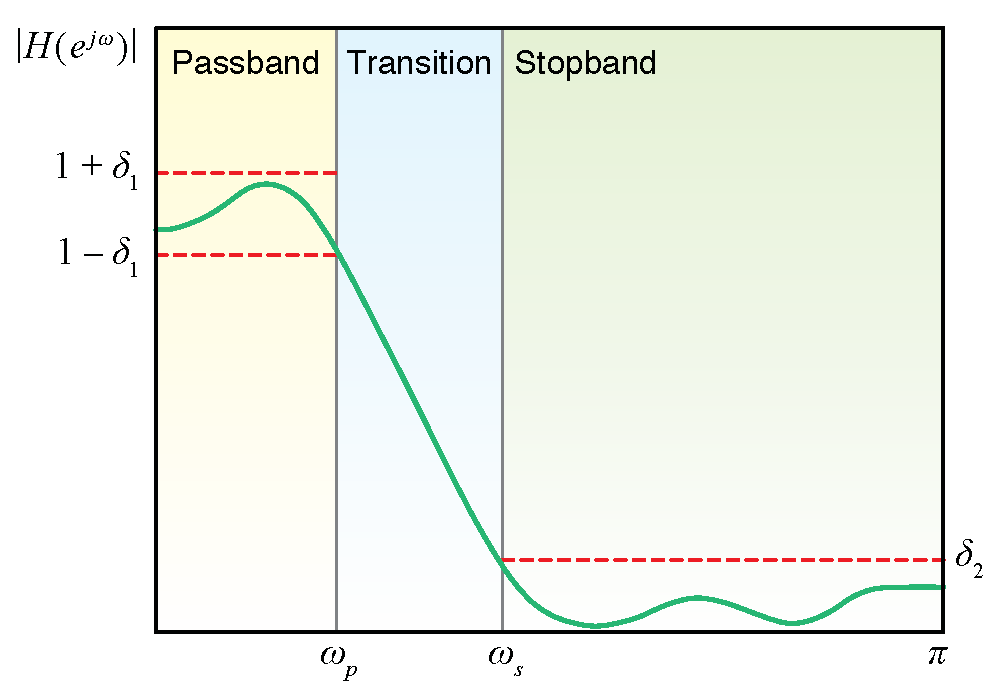
\includegraphics[scale=0.4]{figures/pdf/figure4.pdf} 
% \caption{Specification for effective frequency response
% for the case of low-pass filter. (the discrete-time system).}
% \end{center}   
% \end{figure}


% A Type I Chebyshev filter has an equiripple characteristic in the passband and varies monotonically in the stopband. An elliptic filter is equiripple in both the passband and the stopband. All these approximation methods yield digital filters with non-constant group delay or, equivalently, non-linear phase. The greatest deviation from the constant group delay occurs, in all, cases at the edge of the passband or in the transition band. If phase linearity is not an issue, then elliptic approximation yields the lowest order system function, and therefore elliptic filters will generally require the least computation to implement a given filter specification \citep{Oppenheim_1989}. Altogether, the primary advantage of IIR filters over FIR filters is that the former typically meet a given set of specifications with a much lower filter order than its corresponding FIR filter. Although IIR filters have nonlinear phase, data processing using software such as MATLAB is commonly performed at a post-processing stage (offline), and therefore the entire data sequence is available for filtering. This allows one to use non-causal, zero-phase filtering approach by forward and backward filtering (two-pass) the signals (e.g., via the filtfilt function). This process eliminates the nonlinear phase distortion of IIR filters. Here, we adopt this strategy and all of our filters are zero phase. Consequently, we do not address phase variations and concentrate only on amplitude effects.



% \section{Evaluation}
% \subsection{Goodness of fit function}
% It follows from the previous section that designing a filter entails a trade-off between the accuracy of the response of the passband, the transition zone, and the stopband. Different applications will therefore require different methods to assess the efficacy of a filter. The most common alternative for this is to compare the Fourier amplitude spectra. This  evaluation is typically done visually. We, however, seek to define standards that provide a solid reference framework for simulation validation. That is, we are interested in filters that are good for narrow bands at low frequencies and wider bands at higher frequencies, with sharp transition zones (sharp cut off frequency is better), minimum ripples in the passband amplitudes, and with sufficient attenuation in the stopbands (see Figure 4). In the context of the GOF analysis, \citet{Anderson_2004} defined the expression to evaluate the similarity between two Fourier amplitude spectra as:


% % 
% \begin{equation}
%     \label{eq:s}
% 	S \left( p_1,p_2 \right) = 10 \exp \left\{ -\left[ \frac{p_1-p_2}{min \left(p_1,p_2\right)} \right]^2 \right\} 
%     \hspace{0.25em},
% \end{equation}
% % 

% Where $p_1$ and $p_2$ are the frequency amplitude of two waveforms evaluated at every frequency. Since the Fourier amplitude score in Anderson?s GOF method is the least sensitive parameter to filtering, we are interested in using a similar function to evaluate the filters? selection. Eq. (2) decreases monotonically as the difference between the parameters p1 and p2 increases. While this offers a good measure for almost all scales, it cannot characterize the differences when one of the parameters vanishes (becomes zero). This is important because in order to quantify the efficacy of the filtering process, we also need to consider the values in the stop band, which should be compared to zero. \citet{Khoshenvis_2015} defined complementary goodness of fit function for outside of the pass band where the ideal filter?s magnitude response is zero. 

% % 
% \begin{equation} 
%     \label{eq:s-modified}
%     S \left( p_1,p_2 \right) = 10 \exp \left\{ -\left[ \frac{p_1 - p_2}{F(a)} \right]^2 \right\} 
%     \hspace{0.25em},
% \end{equation}
% % 

% where $F(a)$ is a function of the amplitude inside the passband. The scoring scale defined by Eq. (3) avoids the division by zero and yet offers a signal specific measure of the accuracy of the filter with respect to an ideal filter with amplitude zero in the stopbands. We use Eq. (2) and Eq. (3) to evaluate the efficacy of filters by comparing the Fourier amplitudes of filtered signals with respect to the result that would be expected from an ideal filter, where the amplitude in the passband is the same amplitude of the original signal within the cutoff frequencies, and zero elsewhere. 
% Figure 5 shows an example of this comparison and the resulting scores, using Eq. (2) for scoring the amplitude similarity in the passband and Eq. (3) for scoring the filtered signal remnant amplitude in the stopbands. The whole domain for comparing is max 1 Hz above and below the cutoff frequencies. In this study we assumed F(a) is a fraction of the average amplitude inside the band.

% % 
% \begin{equation}
%     F(a) = C *  \mathrm{mean} \left( [f_1,f_2] \right)
%     \hspace{0.25em}.
% \end{equation}
% % 

% The values are computed for each discrete frequency and the final score is the mean of  the score at all frequencies within the comparison range.  

% \begin{figure} [H]
% \begin{center}  
% 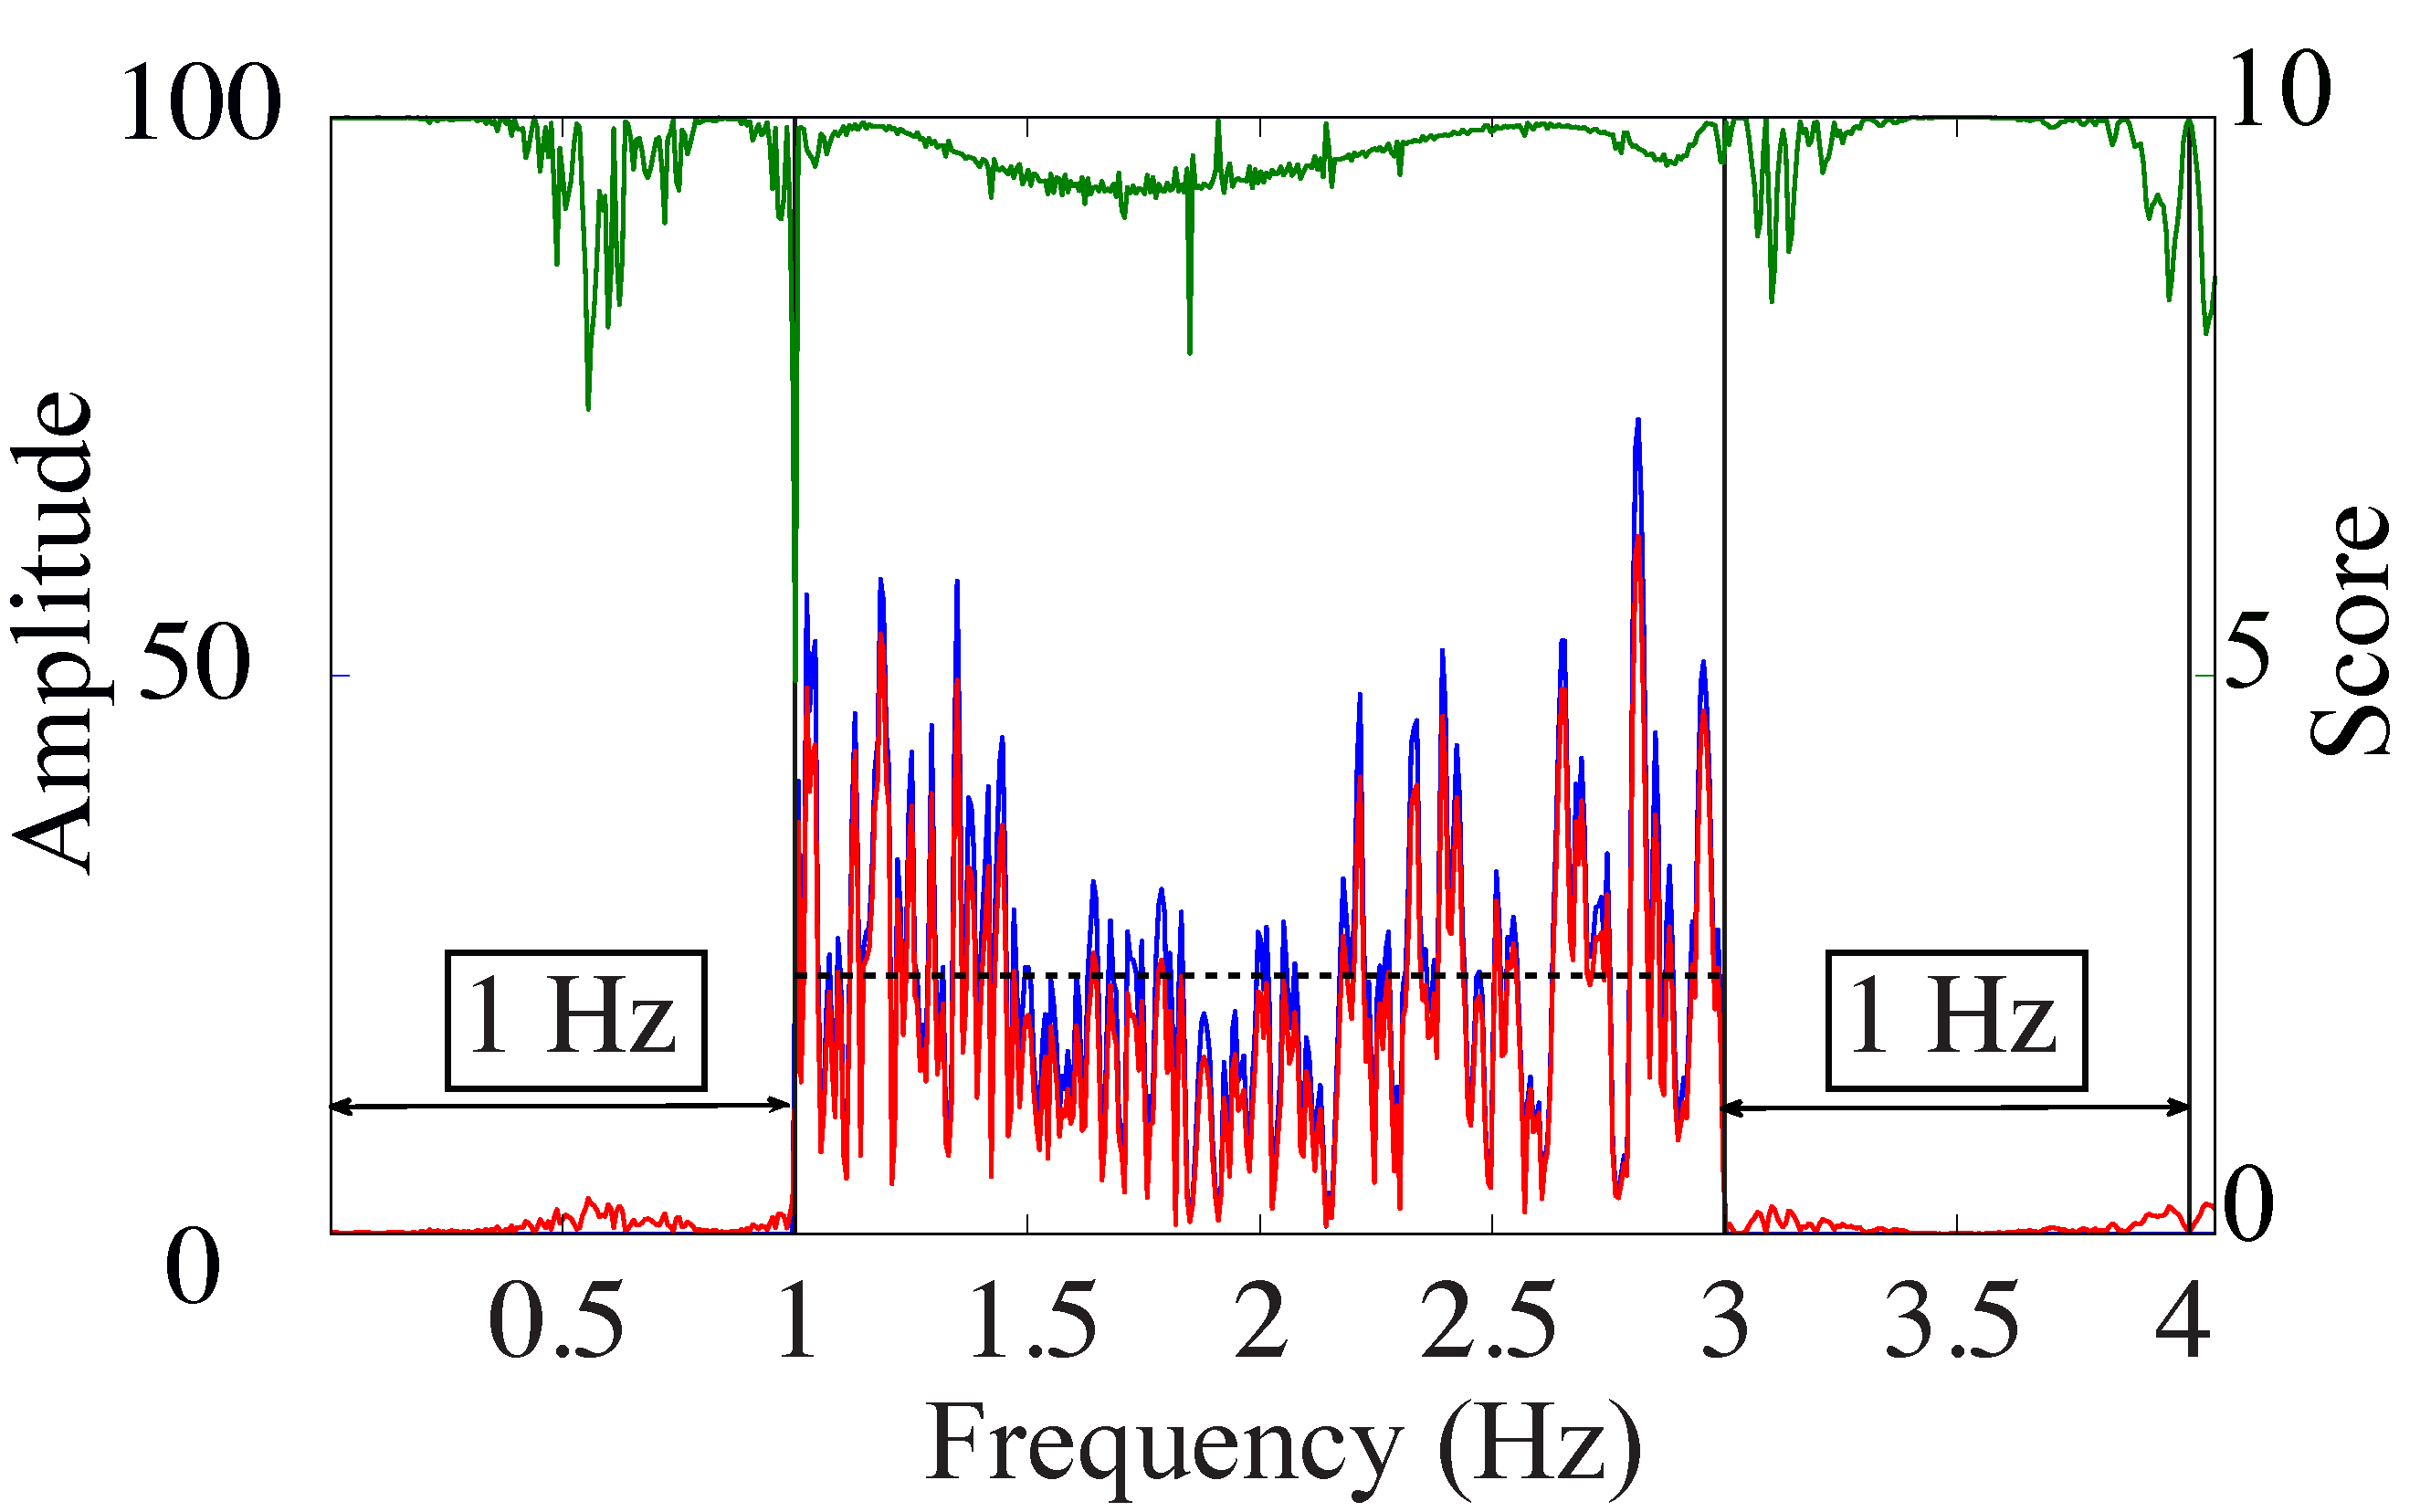
\includegraphics[scale=0.3]{figures/pdf/figure5.pdf} 
% \caption{Evaluation of coherency between the ideal frequency response and filtered signal?s response. Left vertical axes is the amplitude and right vertical axes is the score. The mean of amplitude in the inside section is shown as dashed line.}
% \end{center}   
% \end{figure}


% Figure 6 illustrates the sensitivity of the score with changing $F(a)$. In this study we are looking for making a good balance between inside and outside of the band and non of them are dominant unless because of width. Decreasing the value to very low numbers less than (0.2) will make the score of some points very low, which cause unrealistic low score and will affect the broadband score, whereas  we may have good score inside the band. Very high values (higher than 0.4), will make the score very close to 10. This situation affects the functionality of  cost function of GA alghorithm, and make it less sensitive to the other parameters. Even though these numbers are different for different waveforms but the decreasing pattern is the same. We found that 0.25 * mean of inside the band gives good measure to handle the outside of the band according to the average amplitude of the passband.


% \begin{figure} [H]
% \begin{center}  
% 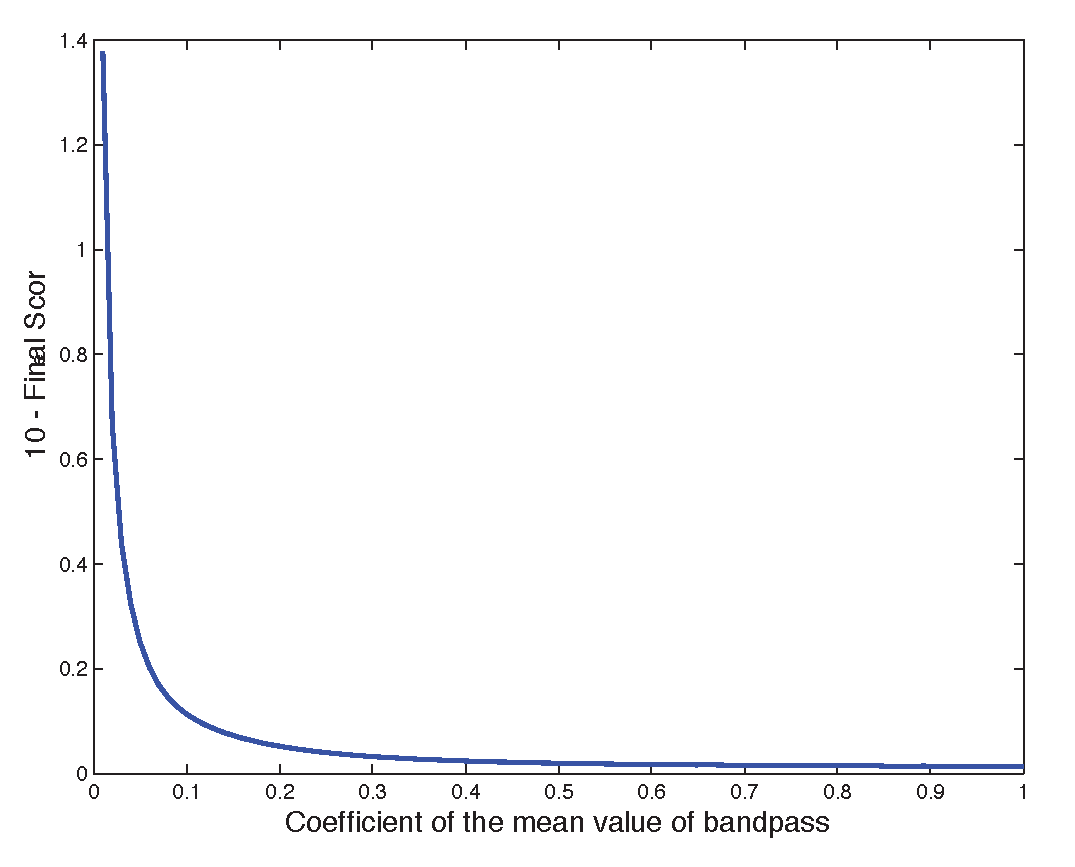
\includegraphics[scale=0.3]{figures/pdf/figure6.pdf} 
% \caption{Sensitivity of final score to the coefficient of  goodness of fit criteria outside of the filtering band.}
% \end{center}   
% \end{figure}



% \subsection{Optimization alghorithm to find the best parameters}

% In this paper we use  Genetic algorithms  (GA) to find the best parameters that results minimum residual than ideal filter. \citet{Holland_1973} introduced genetic algorithms; it is popular till, although it is slower than modified versions; designing efficient algorithm is not objective in this study. GA is not mathematically guided solution to the problem. It is merely a stochastic, discrete, nonlinear, and highly dimensional search algorithm.
% Regarding the trade of entity of ideal filter between paramters, it is common to achevie good score based on different set of parameters,GA has the ability to solve multimodel problem with relative ease. We developed a simple GA  according \citet{Man_1996}. Each population has filters parameters. It is different for different filters. For elliptic filter it has 3 parameters ($LP_O$: order, $LP_RP$: peak to peak passband ripple, $LP_RS$: Stopband attenuation), $LP$ and $HP$ stands for lowpass stands for lowpass and highpass filter. butterworth filter has one parameter (order) and Chebyshev type 1 filter has 2 parameters (Order and peak to peak passband ripple).   The algorithm iteratively defines new populations whose filtered frequency components closely match the ideal frequency component. Every time that new population is generated it went through the evaluation process. In the evaluation process which we call it cost or objective function (according to GA nomencluter), it get the parameters as an input and design a filter based on that parameters. It filter the wave with the designed filter and take Fourier transform. It also take Fourier transform of original waveform and cut the stopnband part in amplitude (see figure 5). Then we evaluate two points at each frequency according to these conditions:


% \begin{equation}
% \left\{\begin{matrix}

% S \left( p_1,p_2 \right) = 10 \exp \left\{ -\left[ \frac{p_1-p_2}{min \left(p_1,p_2\right)} \right]^2 \right\}  \hspace{0.25em}  &  (p_1 > 0.0001) \& (p2 > 0.0001) \\   

%  S \left( p_1,p_2 \right) = 10 \exp \left\{ -\left[ \frac{p_1 - p_2}{F(a)} \right]^2 \right\} \hspace{0.25em} &  (p_1 > 0.0001) \& (p2 < 0.0001) || (p_1 < 0.0001) \& (p2 > 0.0001)\\

% S \left( p_1,p_2 \right) = 10  &  (p_1 < 0.0001) \& (p2 < 0.0001) \\
   
% \end{matrix}\right.
% \end{equation}


% \begin{figure} [H]
% \begin{center}  
% 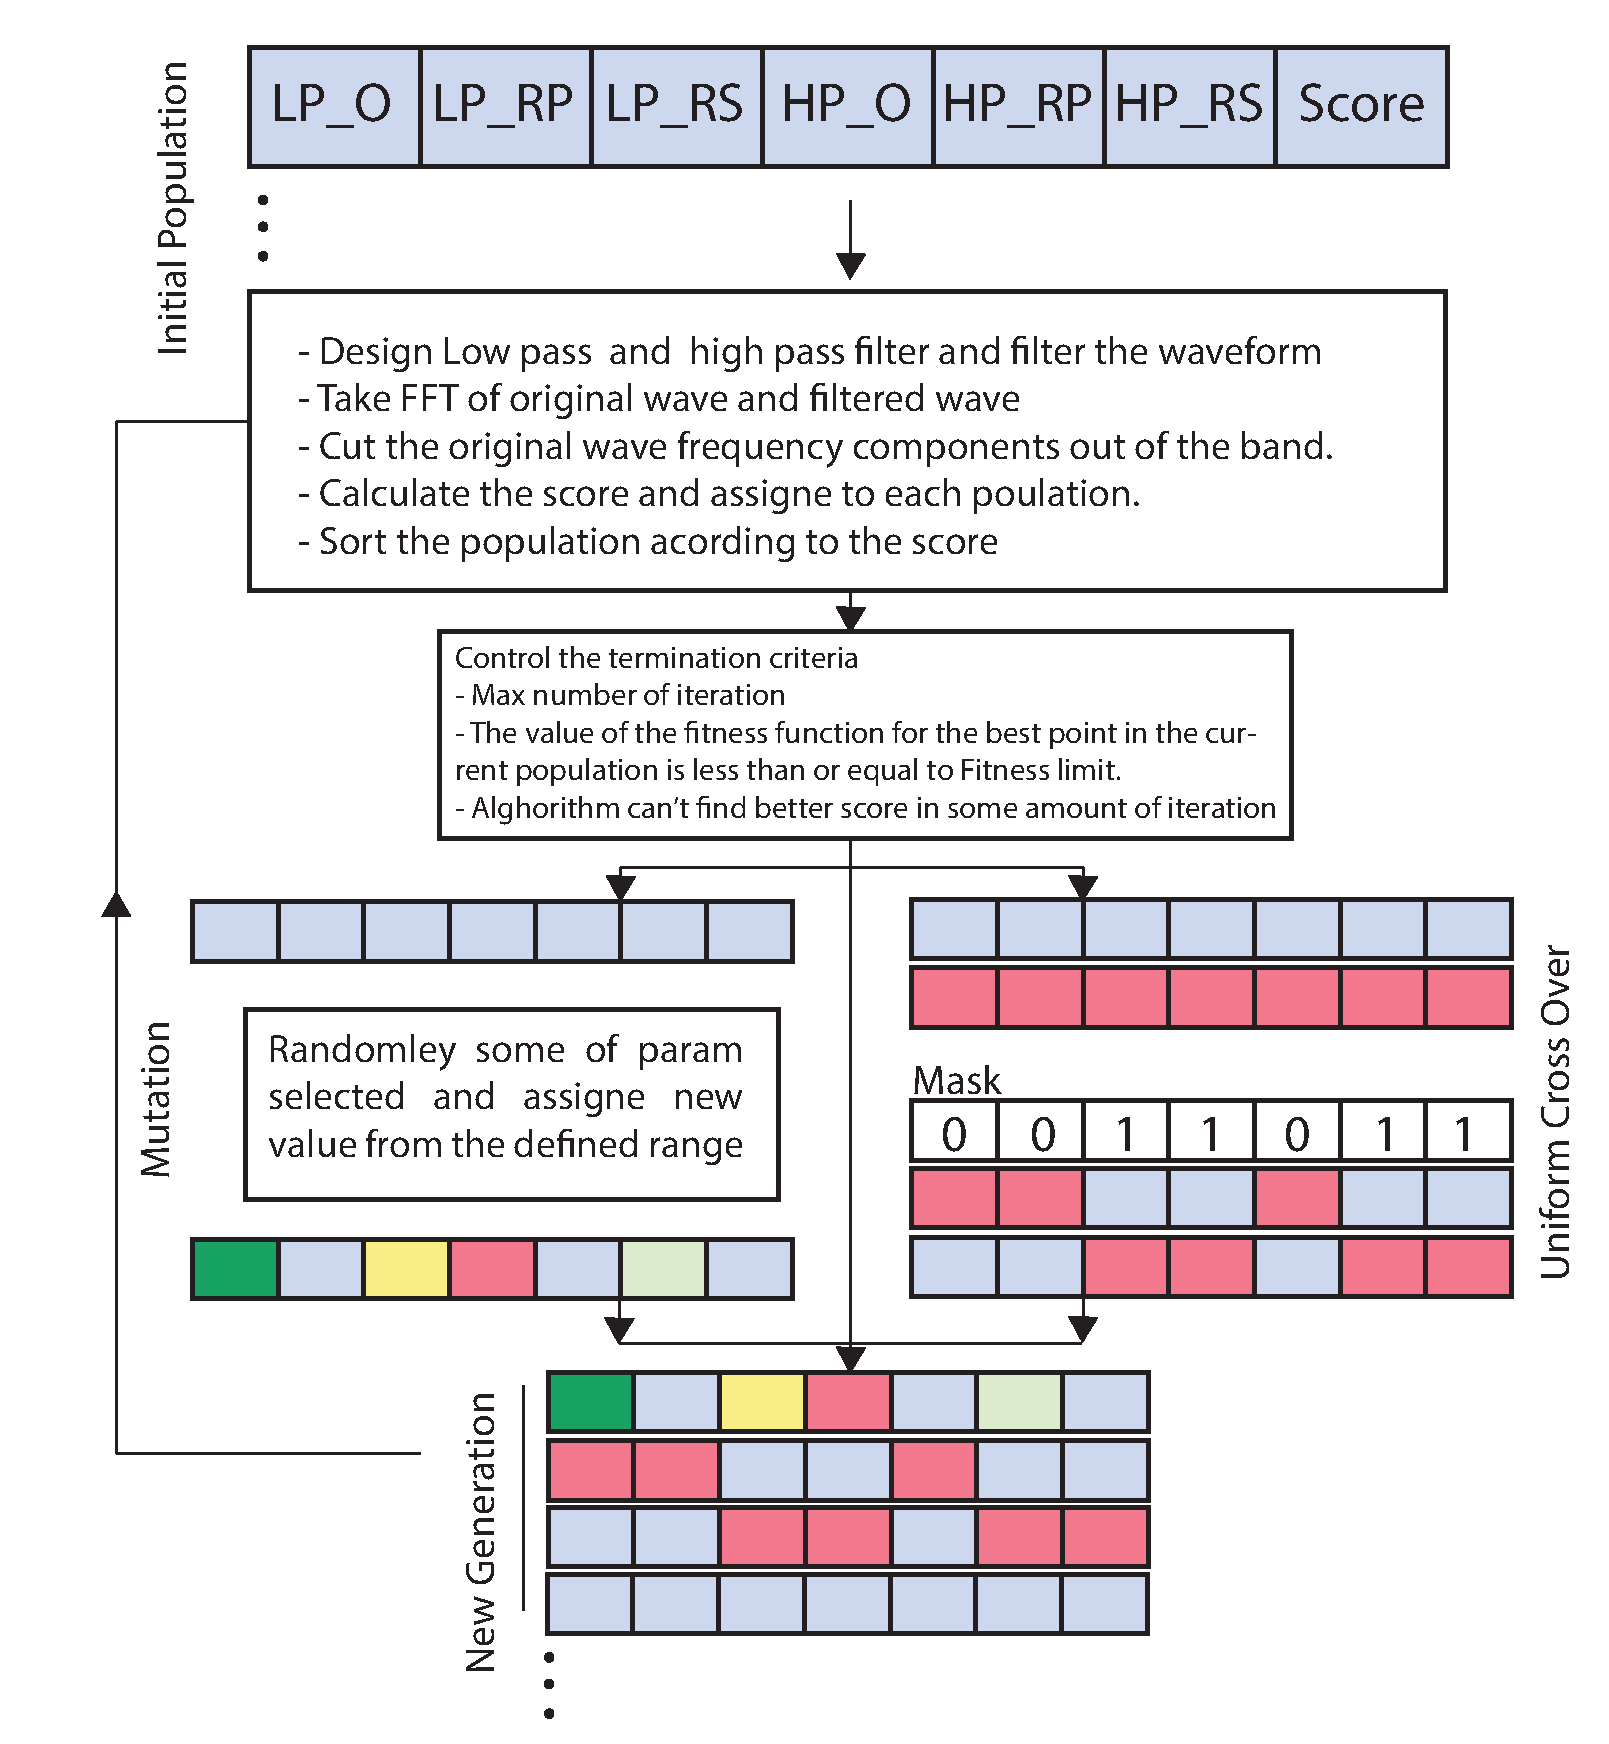
\includegraphics[scale=0.6]{figures/pdf/figure7.pdf} 
% \caption{GA optimization process}
% \end{center}   
% \end{figure}



% \subsection{White noise definition}
% We started to optimize the parameters based on tests on white noises. All numerical signal processing procedures make assumptions about the time series outside of the recorded segments. Time-domain filtering programs assume that the time series is zero on either side of the segment of data being filtered, and frequency-domain filtering using a discrete Fourier transform, as in the FFT, assumes that the time series is periodic, with period equal to the length of the data segments extended with zeros or truncated to a number of points equal to a power of two. 
% \citet{Converse-1992} suggest the below equation to zeropad the initial and end of the waveform. 




% \begin{equation}
% T{_z{_p{_a{_d}}}} = \frac{1.5n}{f_c}
% \end{equation}

% Where $T(sec)$ is the total length of zeros to be added to the record, $n$ (an integer) is the order of the Butterworth filter, and $f_c$ is the corner frequency. In this study we deal with different kind of filter and different filtering order, nevertheless the effect of abrupt cut of data is not negligible. \citet{Boore_2005} showed that zero padding assuming the Butterwoth filter order is 4, gives trustable wave form in the sense of numerical problem. Practically it is not possible to filter the waveform with corner frequency of 0 Hz. After \citet{Trifunac_1971}  many networks in order to do baseline correction, high pass filter the waveform  with 0.05 Hz corner frequency ( e.g. cosmos-format). Even though for numerical models, theoretically achieving very close numbers to zero is possible, we wanted to make all analysis consistent for data and synthetic. We choose $f_c= 0.05$ Hz as a smallest highpass corner frequency. So the added time will be 120 s. We add 60 sec of zero pads before and after the data. We defined the 60 white noises with maximum 50 Hz frequency. The total time of data is 100s, which with zero pad part totally will be 220s. We also used Gaussian window ($\alpha$=4) according to equation (7) to taper the data. 

% \begin{equation}
% \omega{_({_n{_)}}} = e ^ {\frac{-1}{2}(\alpha \frac{n}{\frac{N}{2}})^2}
% \end{equation}

% Figure 8 shows one the waveforms.

% \begin{figure} [H]
% \begin{center}  
% 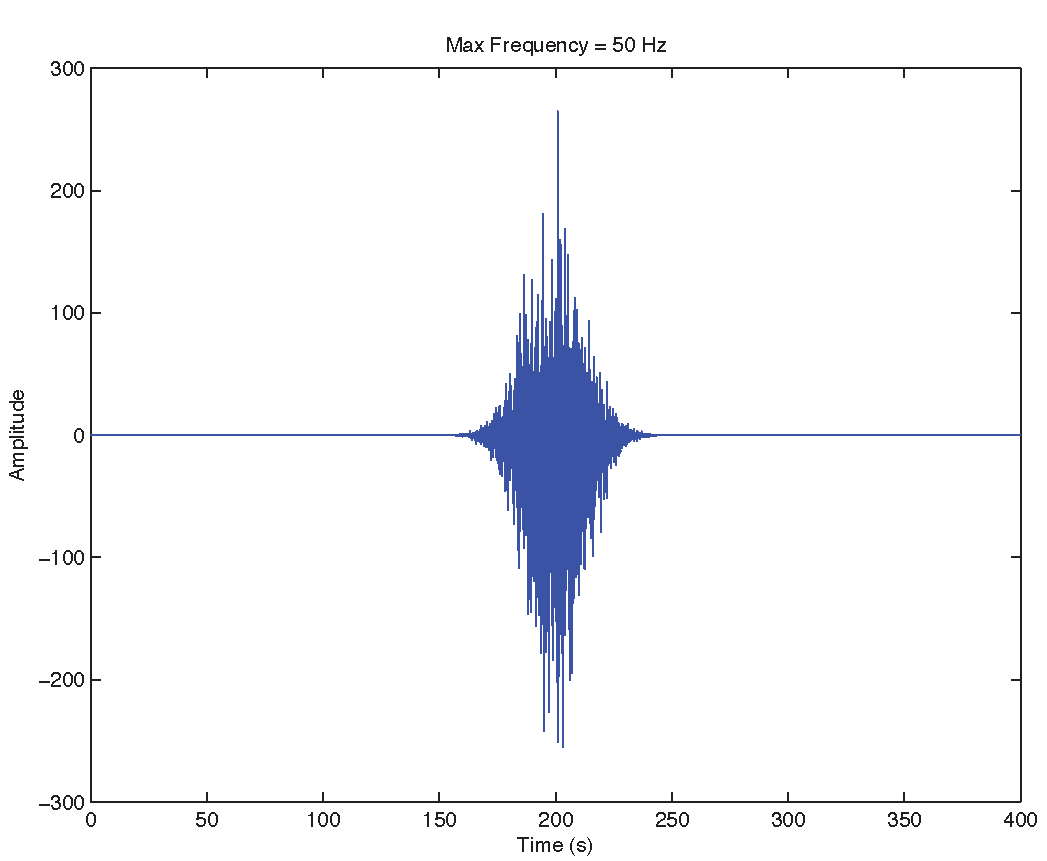
\includegraphics[scale=0.6]{figures/pdf/figure8.pdf} 
% \caption{Test white noise (\textcolor{red!50!black}{time is not correct)}}
% \end{center}   
% \end{figure}

% \section{Filter selection}
% We did a test on one of waveforms for different kind of filters, filtering order (low and high pass), and bandwidth. Even though the optimization algorithm can find the best solution at very early iterations, We deactivate all termination criteria except the iteration to have  common sense of evaluation of all procedures. It is easily seen that elliptic filter both for highpass then lowpass and vice versa gives the best results. Figure 8 shows the results. Butterworth filter gives very close score to elliptic bandpass filter at [0.05,0.25] band, because according to evaluation method there isn?t enough frequency out of band to evaluate. 


% \begin{figure} [H]
% \begin{center}  
% 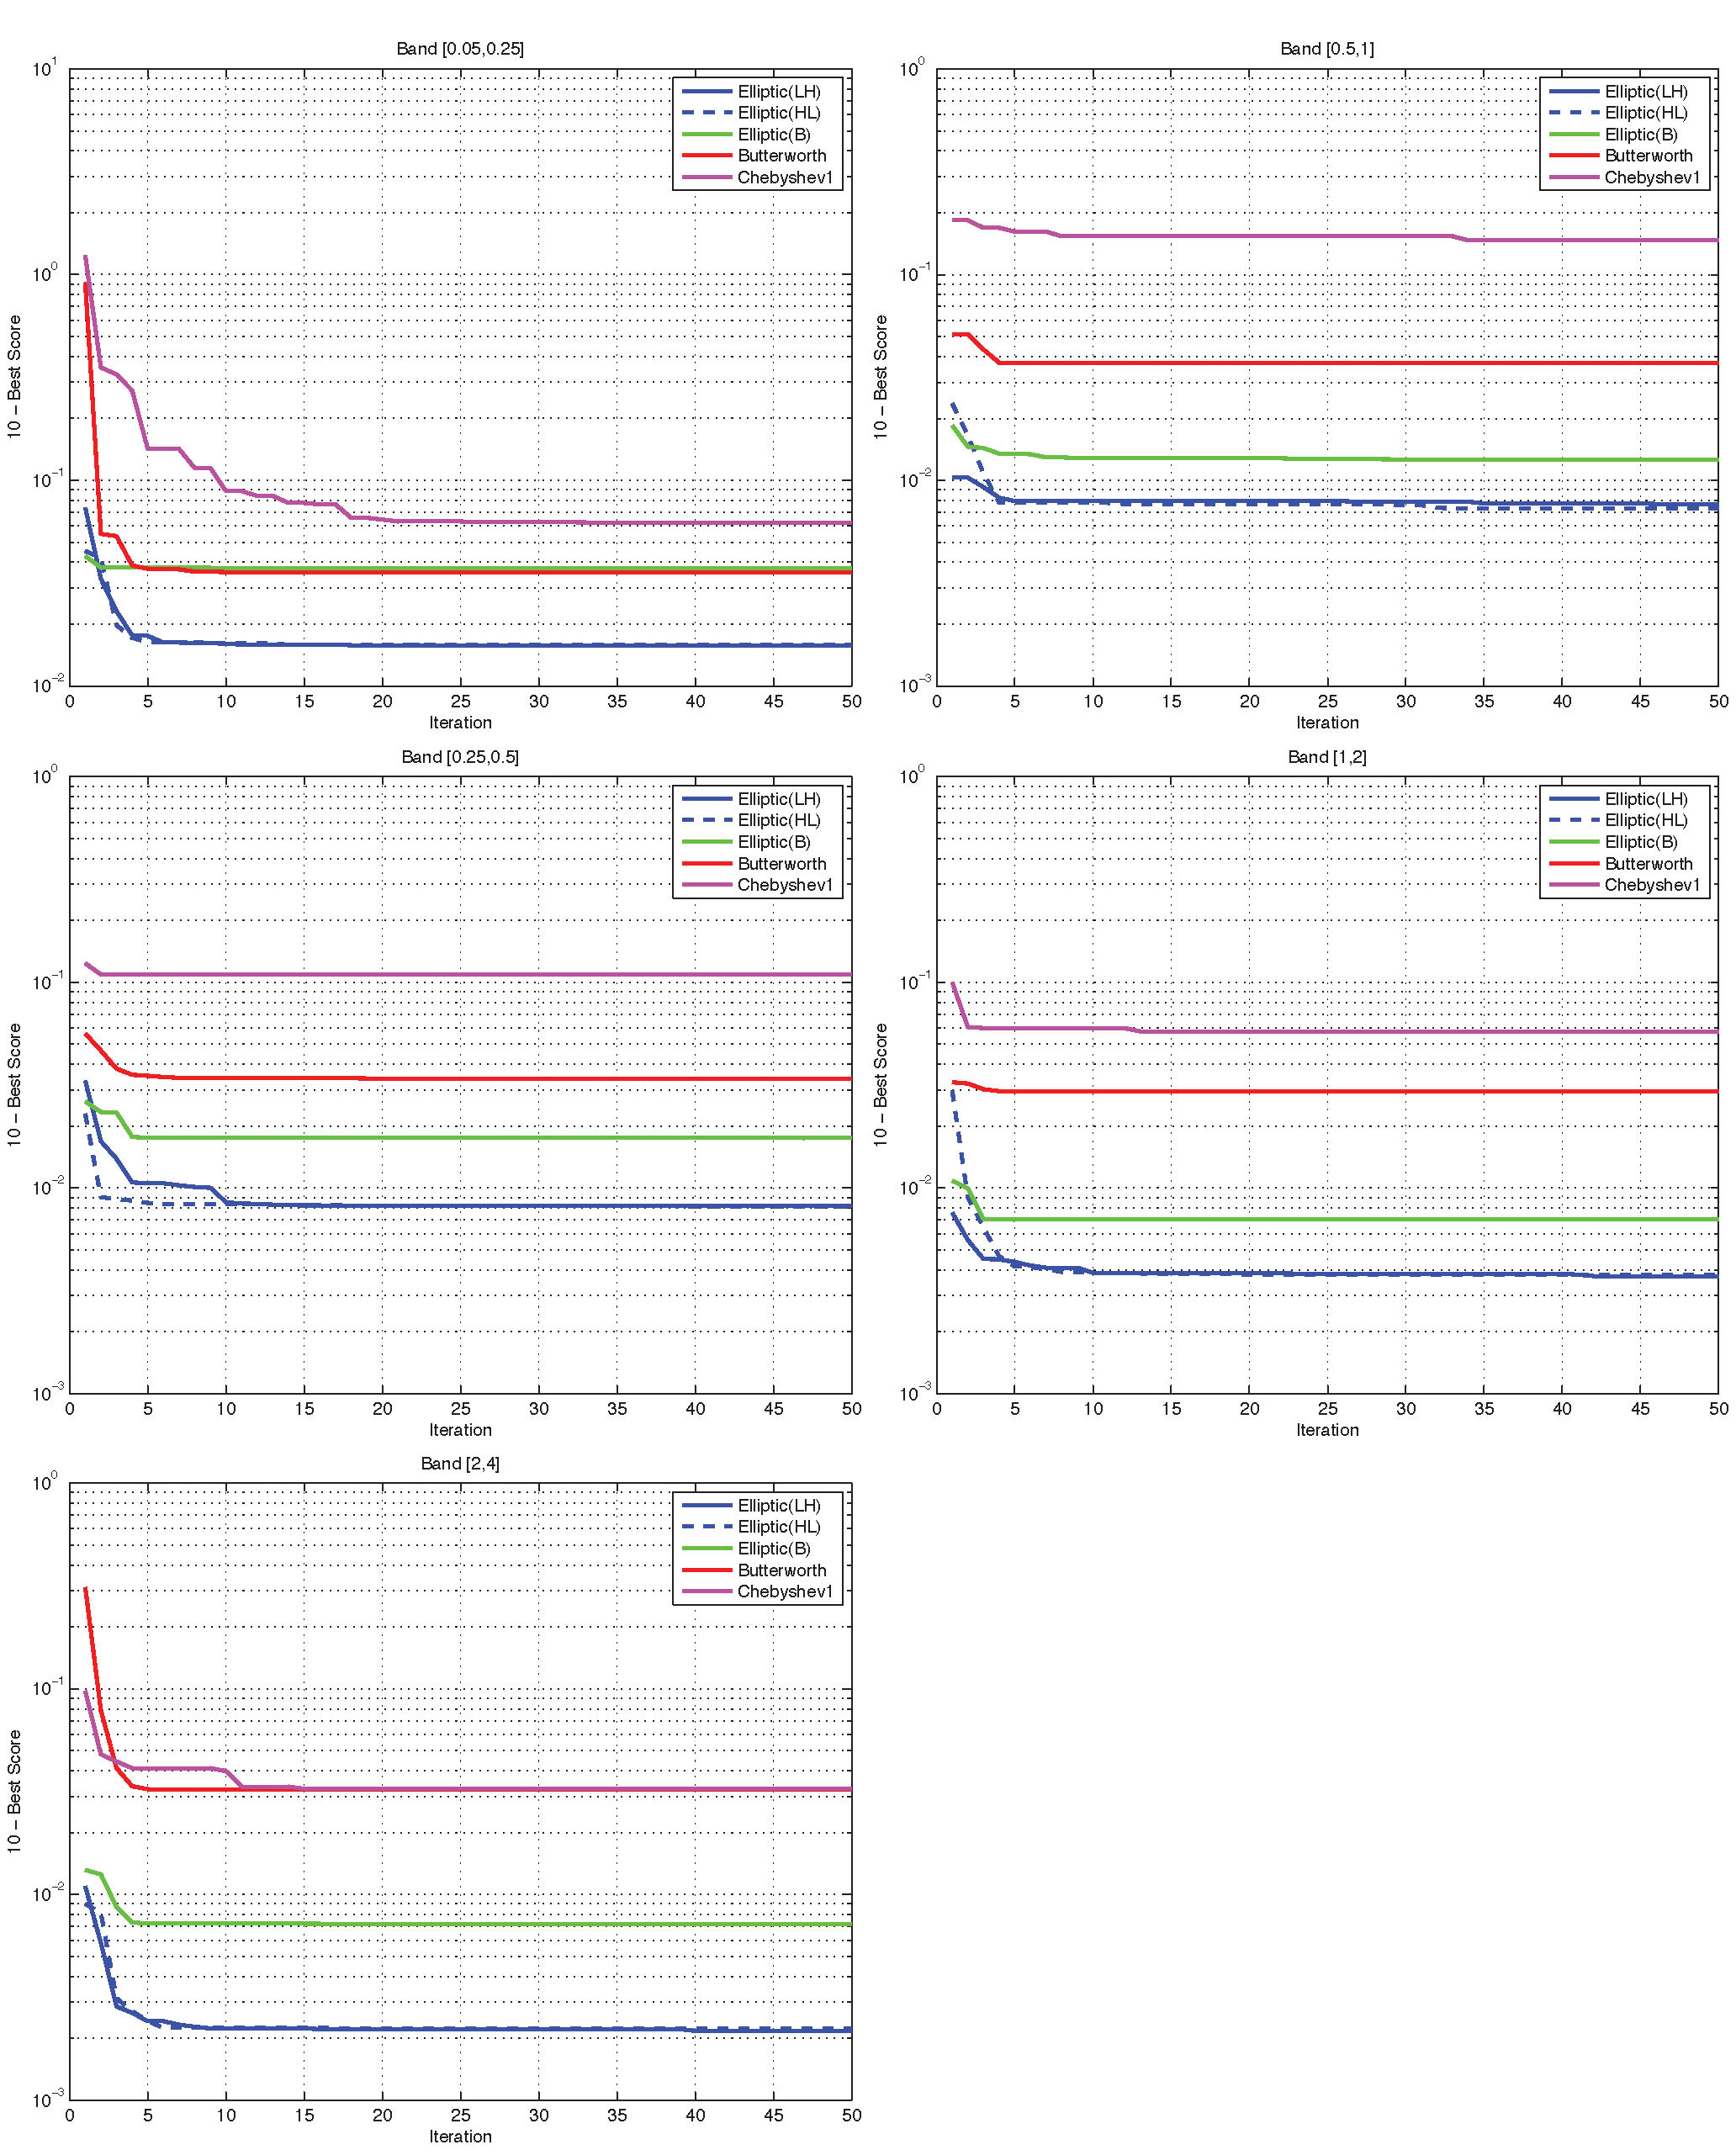
\includegraphics[scale=0.6]{figures/pdf/figure9.pdf} 
% \caption{Variation of the best score in 50 iterations.}
% \end{center}   
% \end{figure}




% \newpage

% %\section*{References}

% {
% \renewcommand{\bibname}{}
% \bibliographystyle{ascelike}
% \bibliography{references}
% }

\setlength{\bibsep}{0pt}
\bibliographystyle{mybssabib}
{\small\bibliography{references}}

